\section{Evolvability}

\begin{frame}{The Evolvability Conundrum}
How can natural selection ``favor properties that may prove useful to a given lineage in the future, but have no present adaptive function''? \cite{Pigliucci2008IsEvolvable}
\end{frame}

\begin{frame}{The Evolvability Conundrum}
Two views of evolvability
\begin{itemize}
  \item evolvability as the ability to generate heritable variation
    \begin{itemize}
      \item individual evolvability
      \item population evolvability
    \end{itemize}
  \item evolvability as bias to the evolutionary search
  \begin{itemize}
    \item regularity
    \item acquired evolvability
  \end{itemize}
\end{itemize}
\end{frame}

\begin{frame}{Evolvability}
\begin{figure}
 \centering
    \begin{subfigure}[b]{0.5\textwidth}
        \centering
    	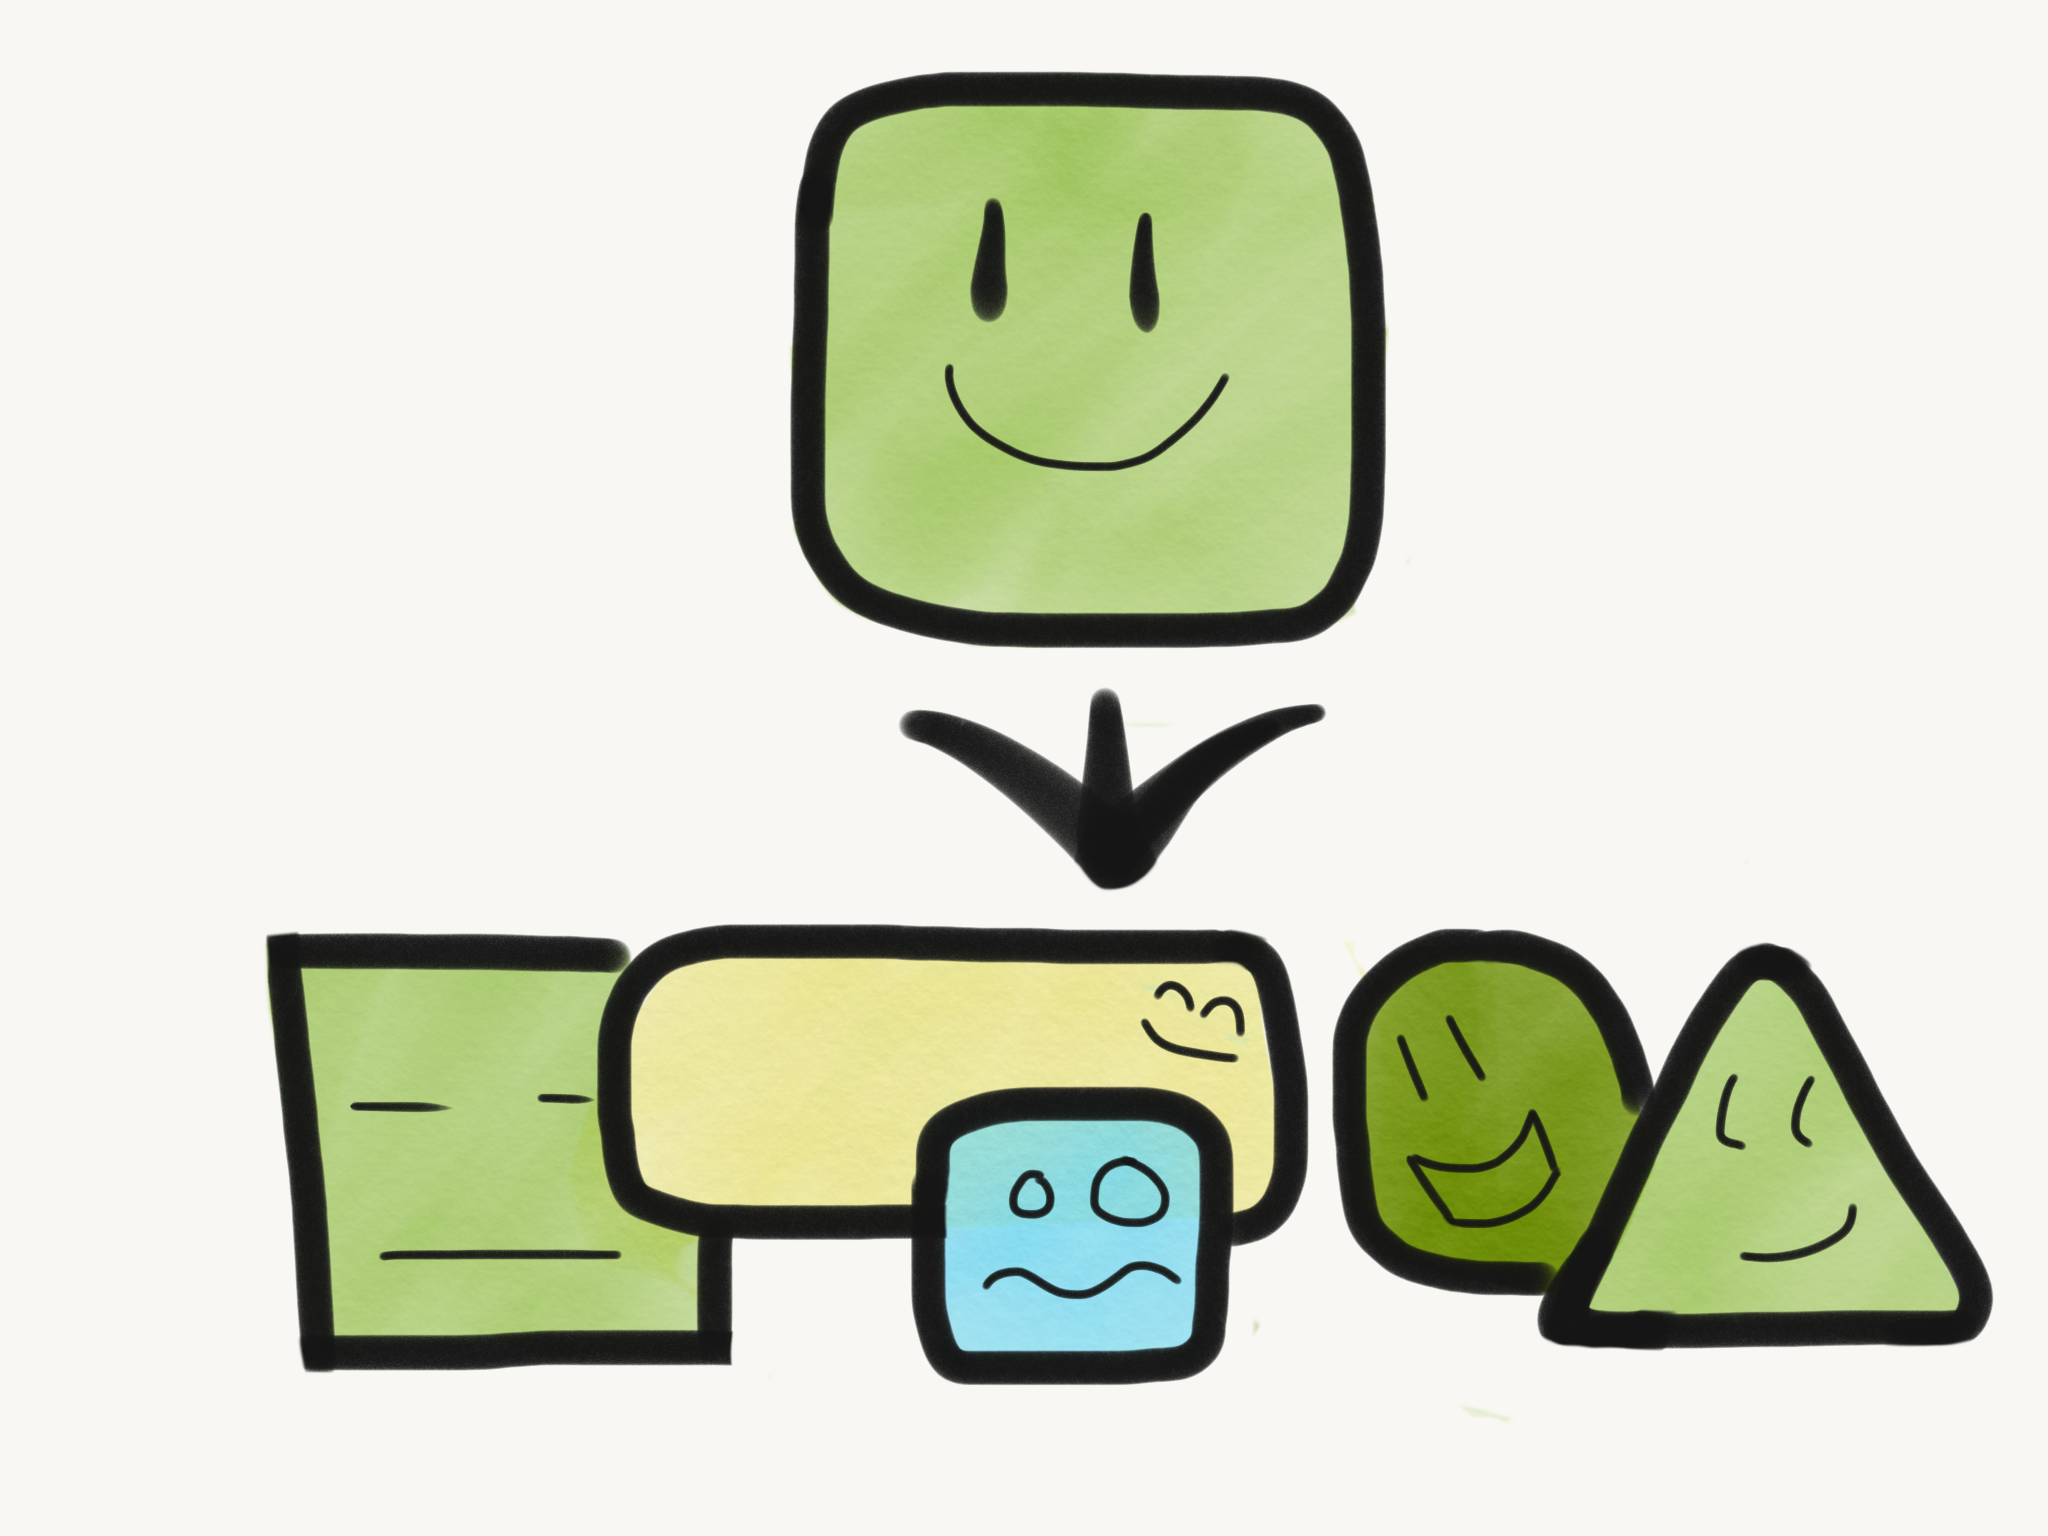
\includegraphics[width=\textwidth]{img/individual_evolvability.png}
        \caption{high individual evolvability}
        \label{subfig:canalization}
    \end{subfigure}%
    \hfill
    \begin{subfigure}[b]{0.5\textwidth}
        \centering
        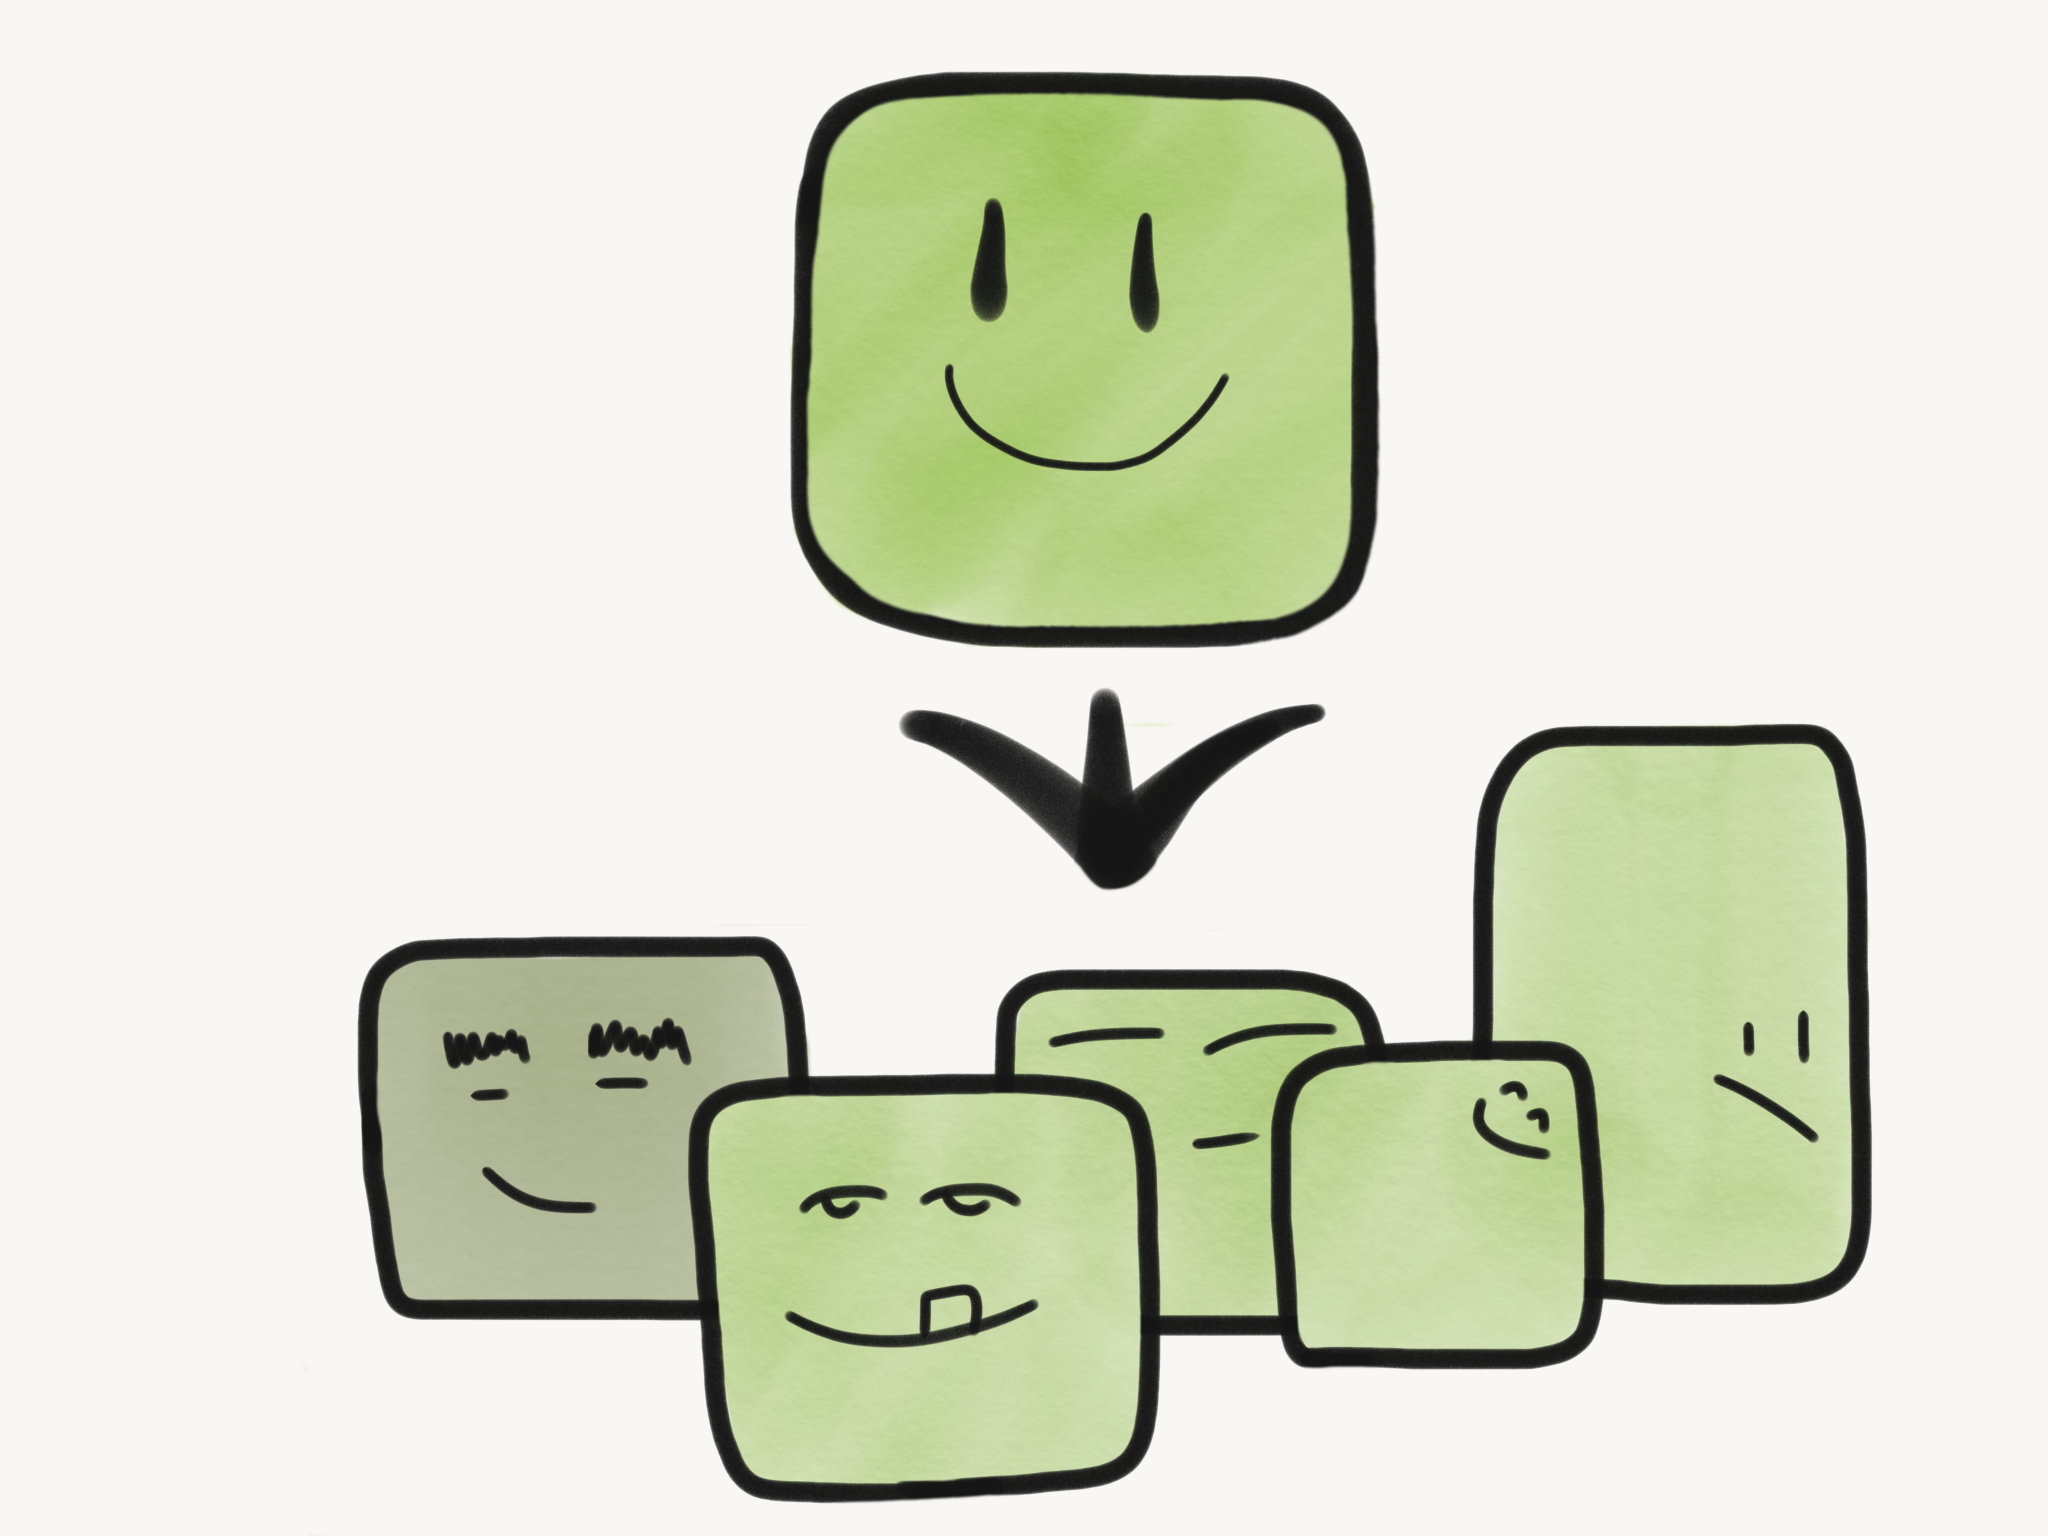
\includegraphics[width=\textwidth]{img/low_individual_evolvability.png}
        \caption{low individual evolvability}
        \label{subfig:no_canalization}
    \end{subfigure}
 	\captionsetup{singlelinecheck=off,justification=raggedright}
    \vspace{-4ex}
  \captionsetup{singlelinecheck=off,justification=raggedright}
  \caption{evolvability as heritable variation}
\end{figure}
\end{frame}


\begin{frame}{Evolvability}
\begin{figure}
 \centering
    \begin{subfigure}[b]{0.5\textwidth}
        \centering
    	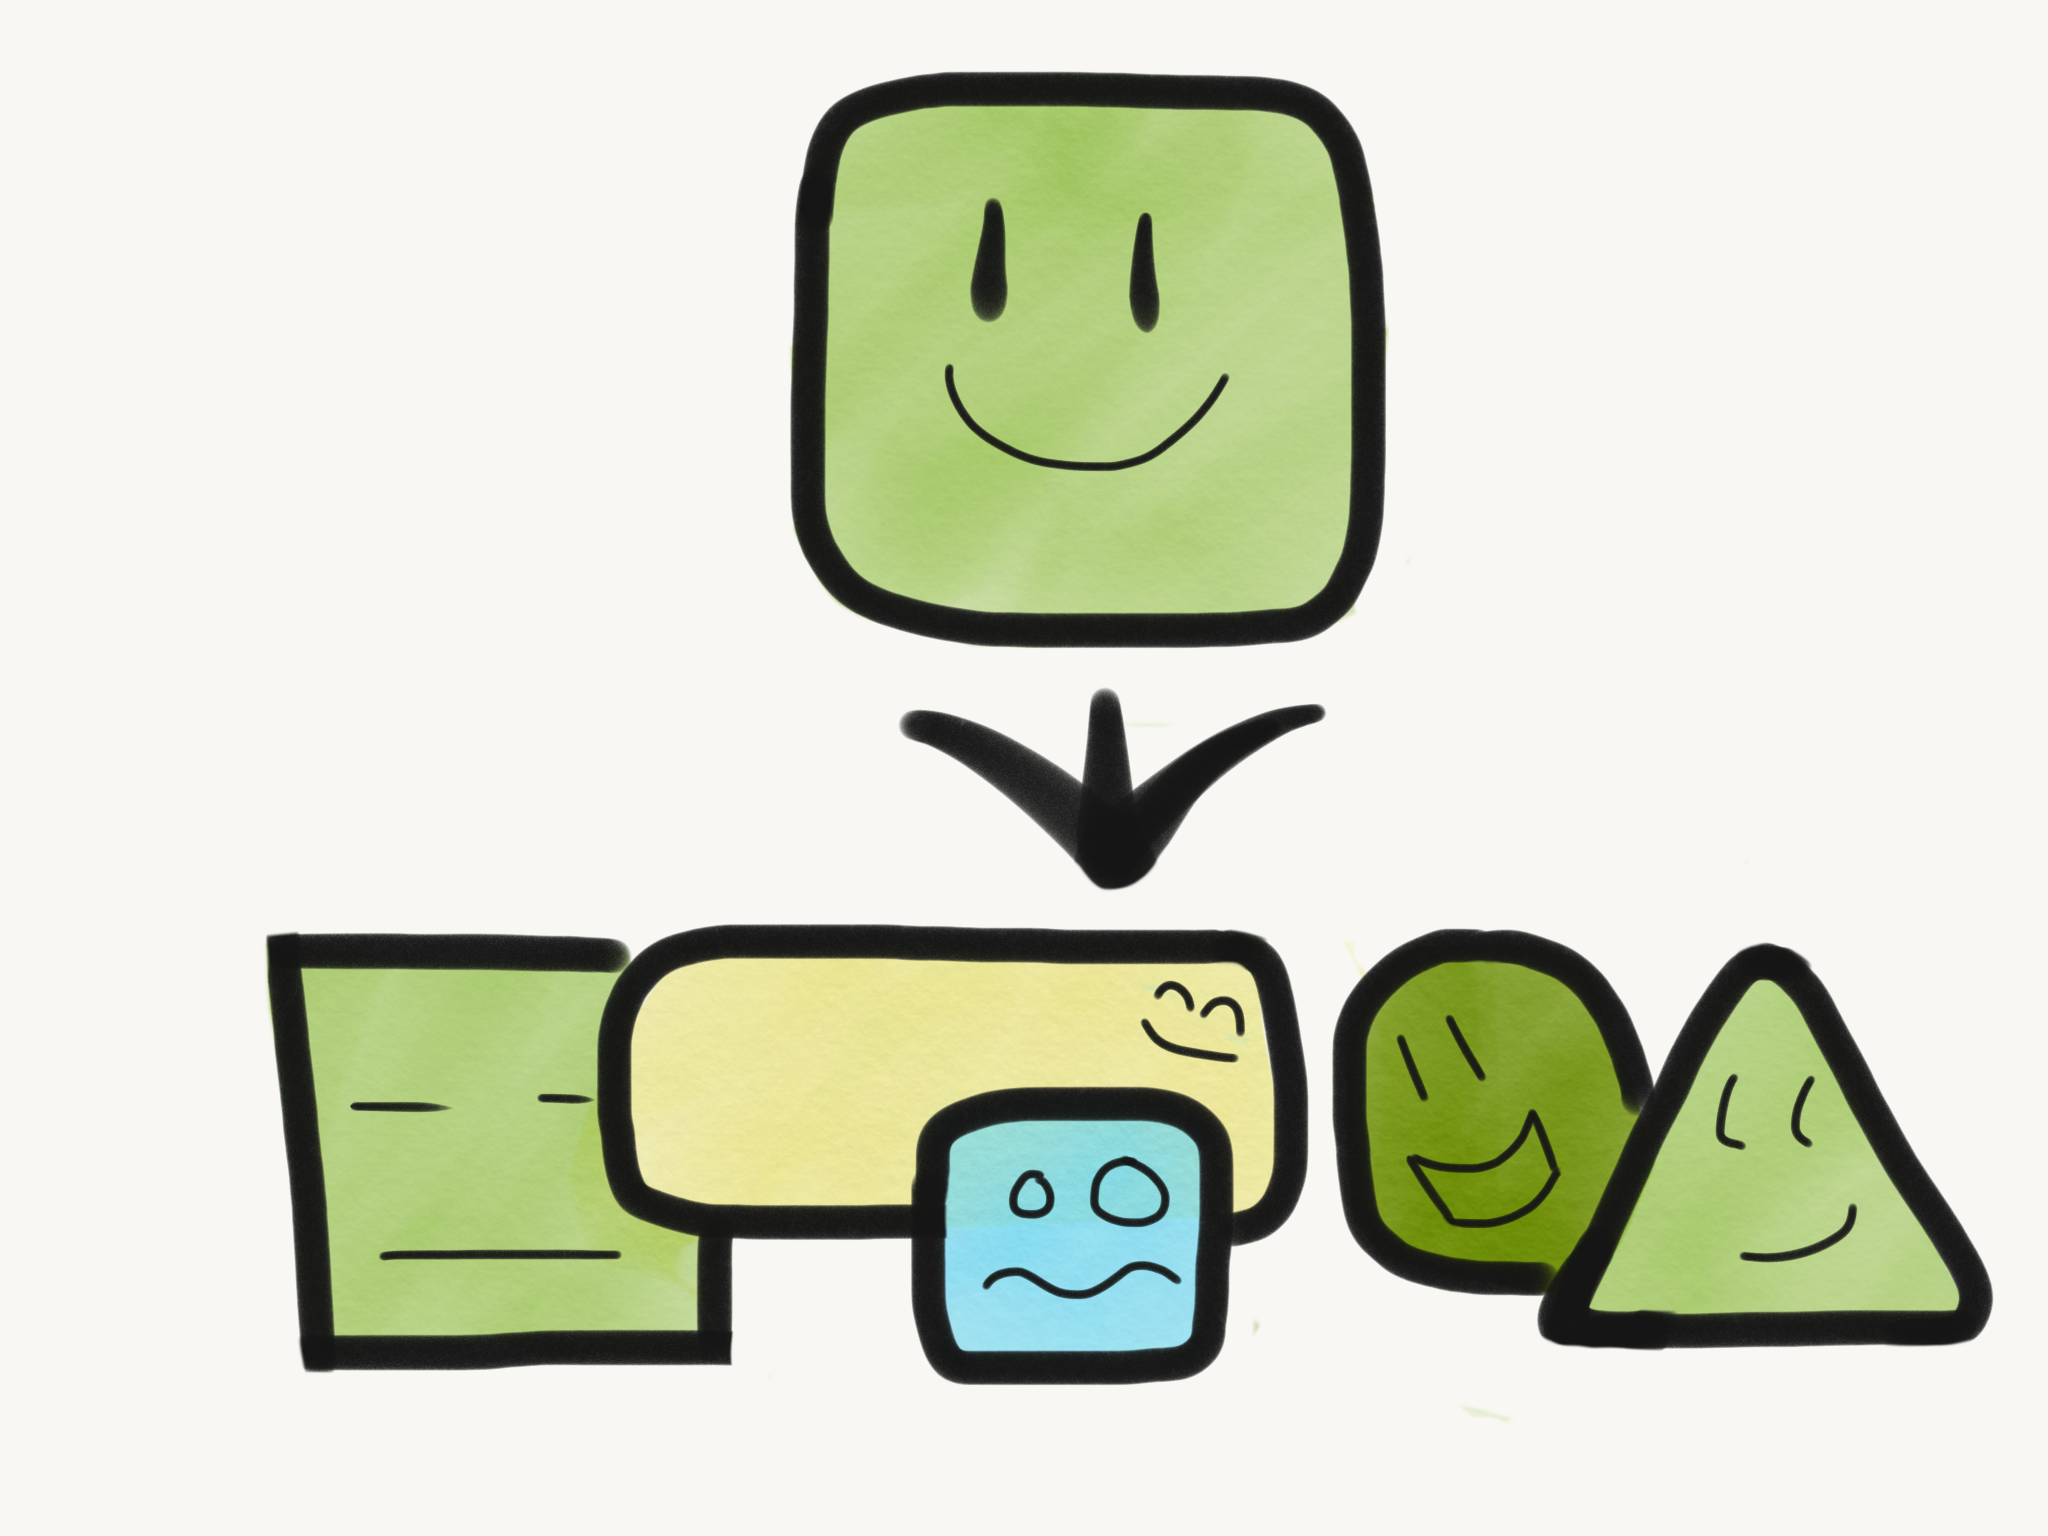
\includegraphics[width=\textwidth]{img/individual_evolvability.png}
        \caption{individual evolvability}
        \label{subfig:individual_evolvability}
    \end{subfigure}%
    \hfill
    \begin{subfigure}[b]{0.5\textwidth}
        \centering
        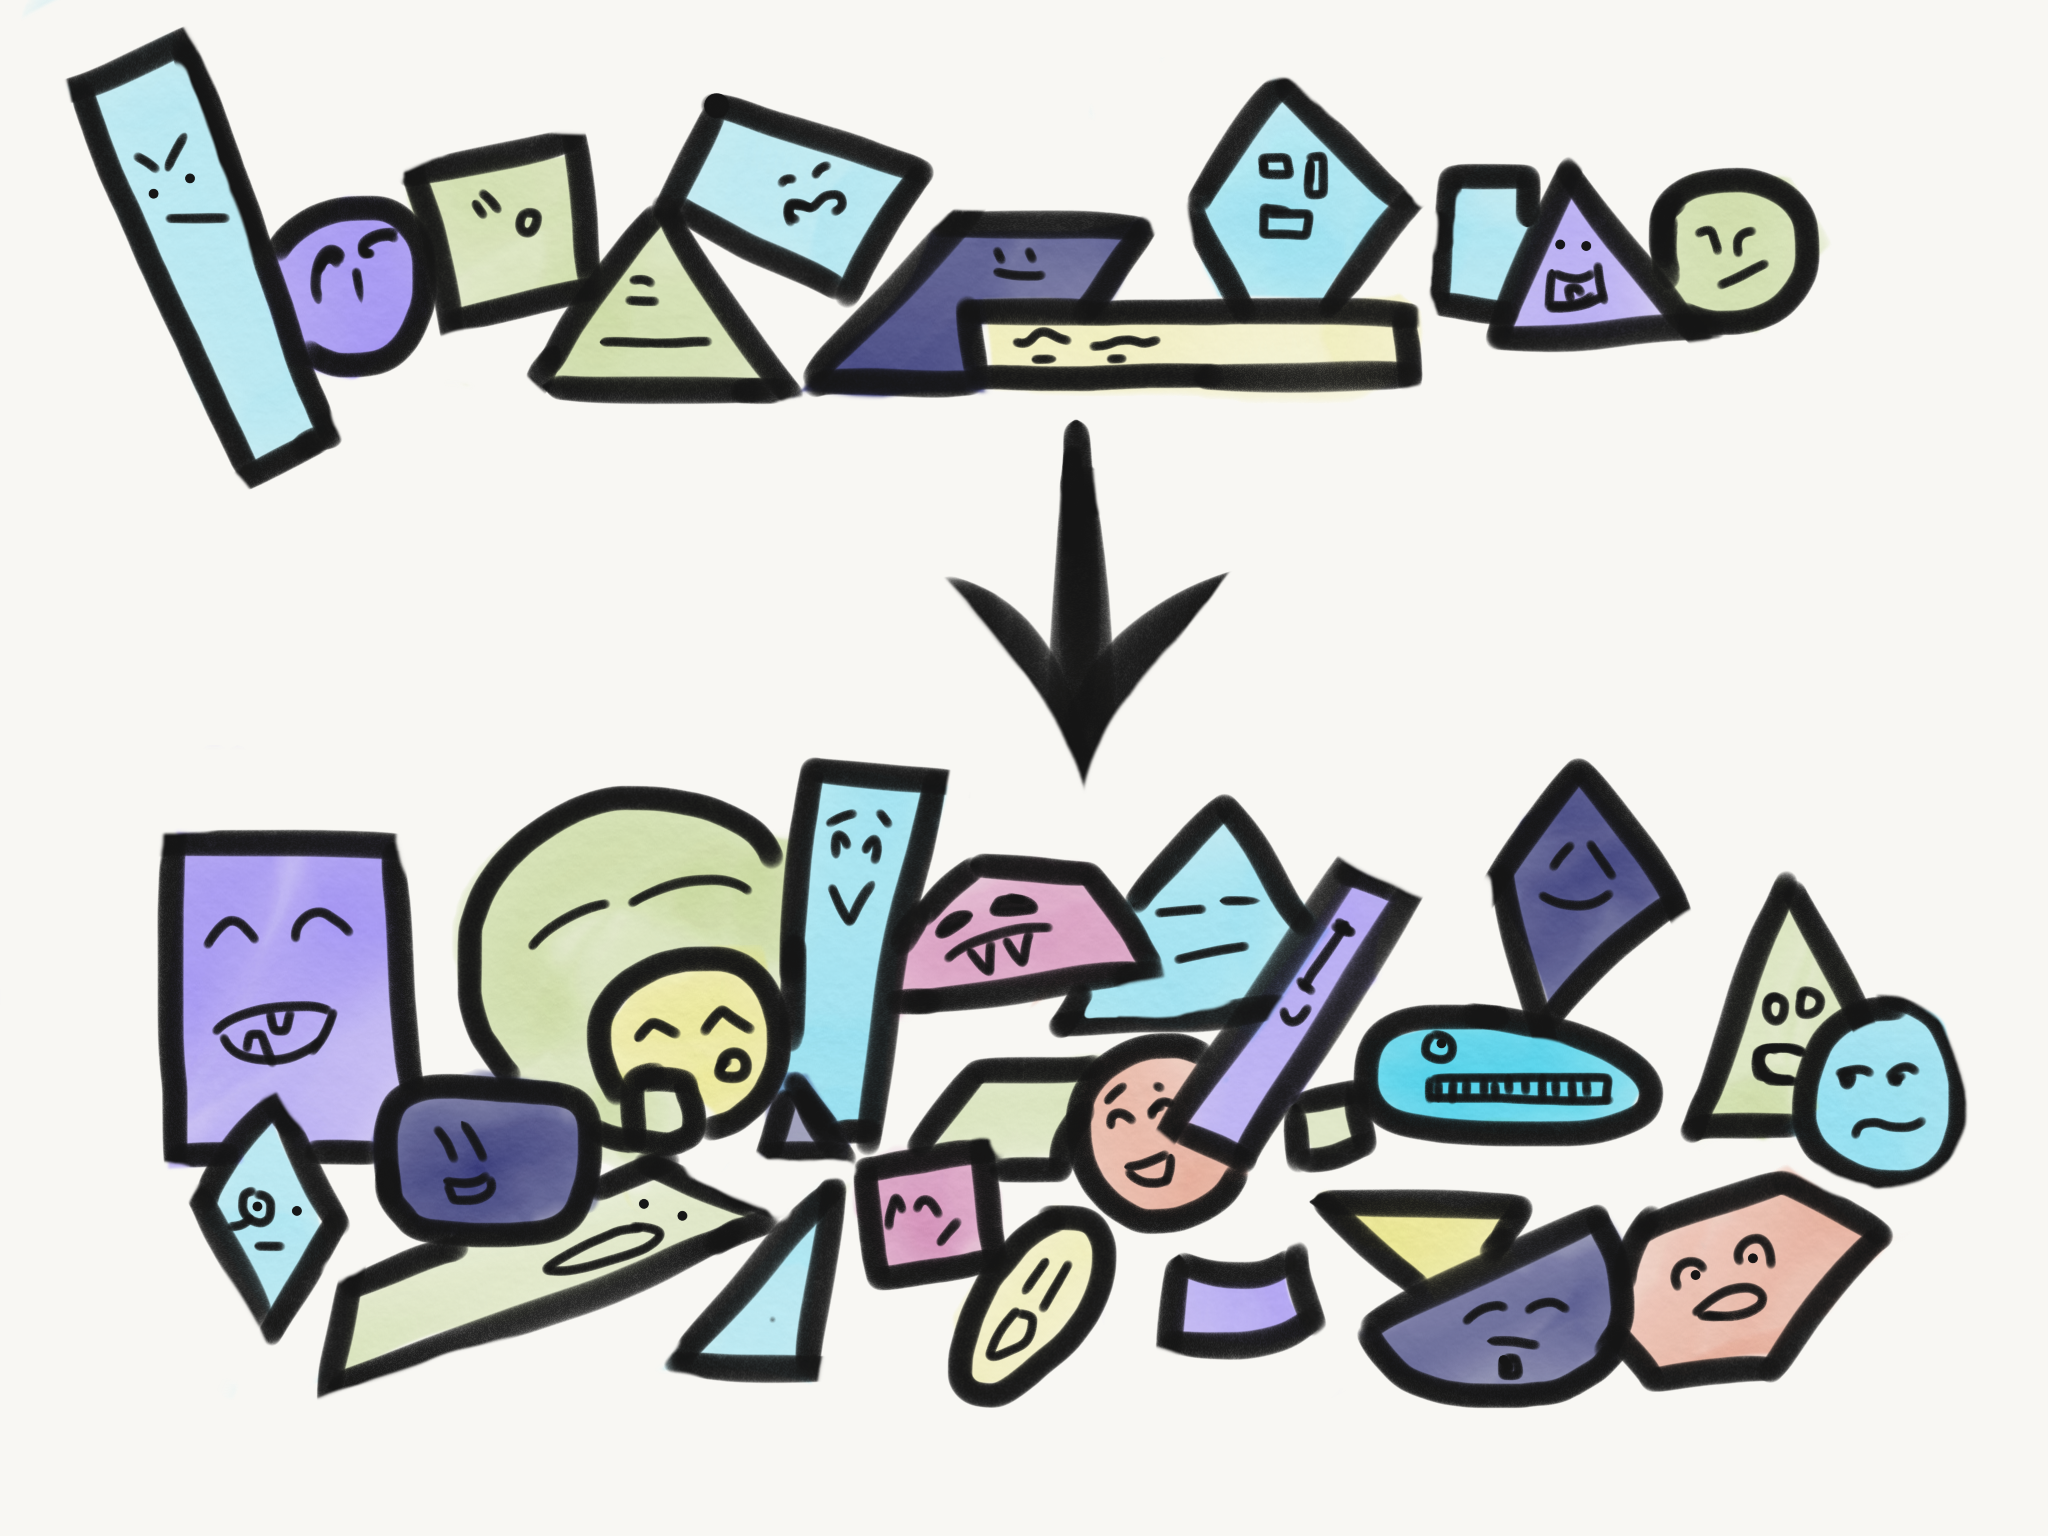
\includegraphics[width=\textwidth]{img/population_evolvability.png}
        \caption{population evolvability}
        \label{subfig:population_evolvability}
    \end{subfigure}
 	\captionsetup{singlelinecheck=off,justification=raggedright}
    \vspace{-4ex}
  \captionsetup{singlelinecheck=off,justification=raggedright}
  \caption{hidden genetic variation}
\end{figure}
\end{frame}

\begin{frame}{Learned Bias: Canalization}
\begin{figure}
  \centering
  \begin{subfigure}[b]{0.5\textwidth}
      \centering
      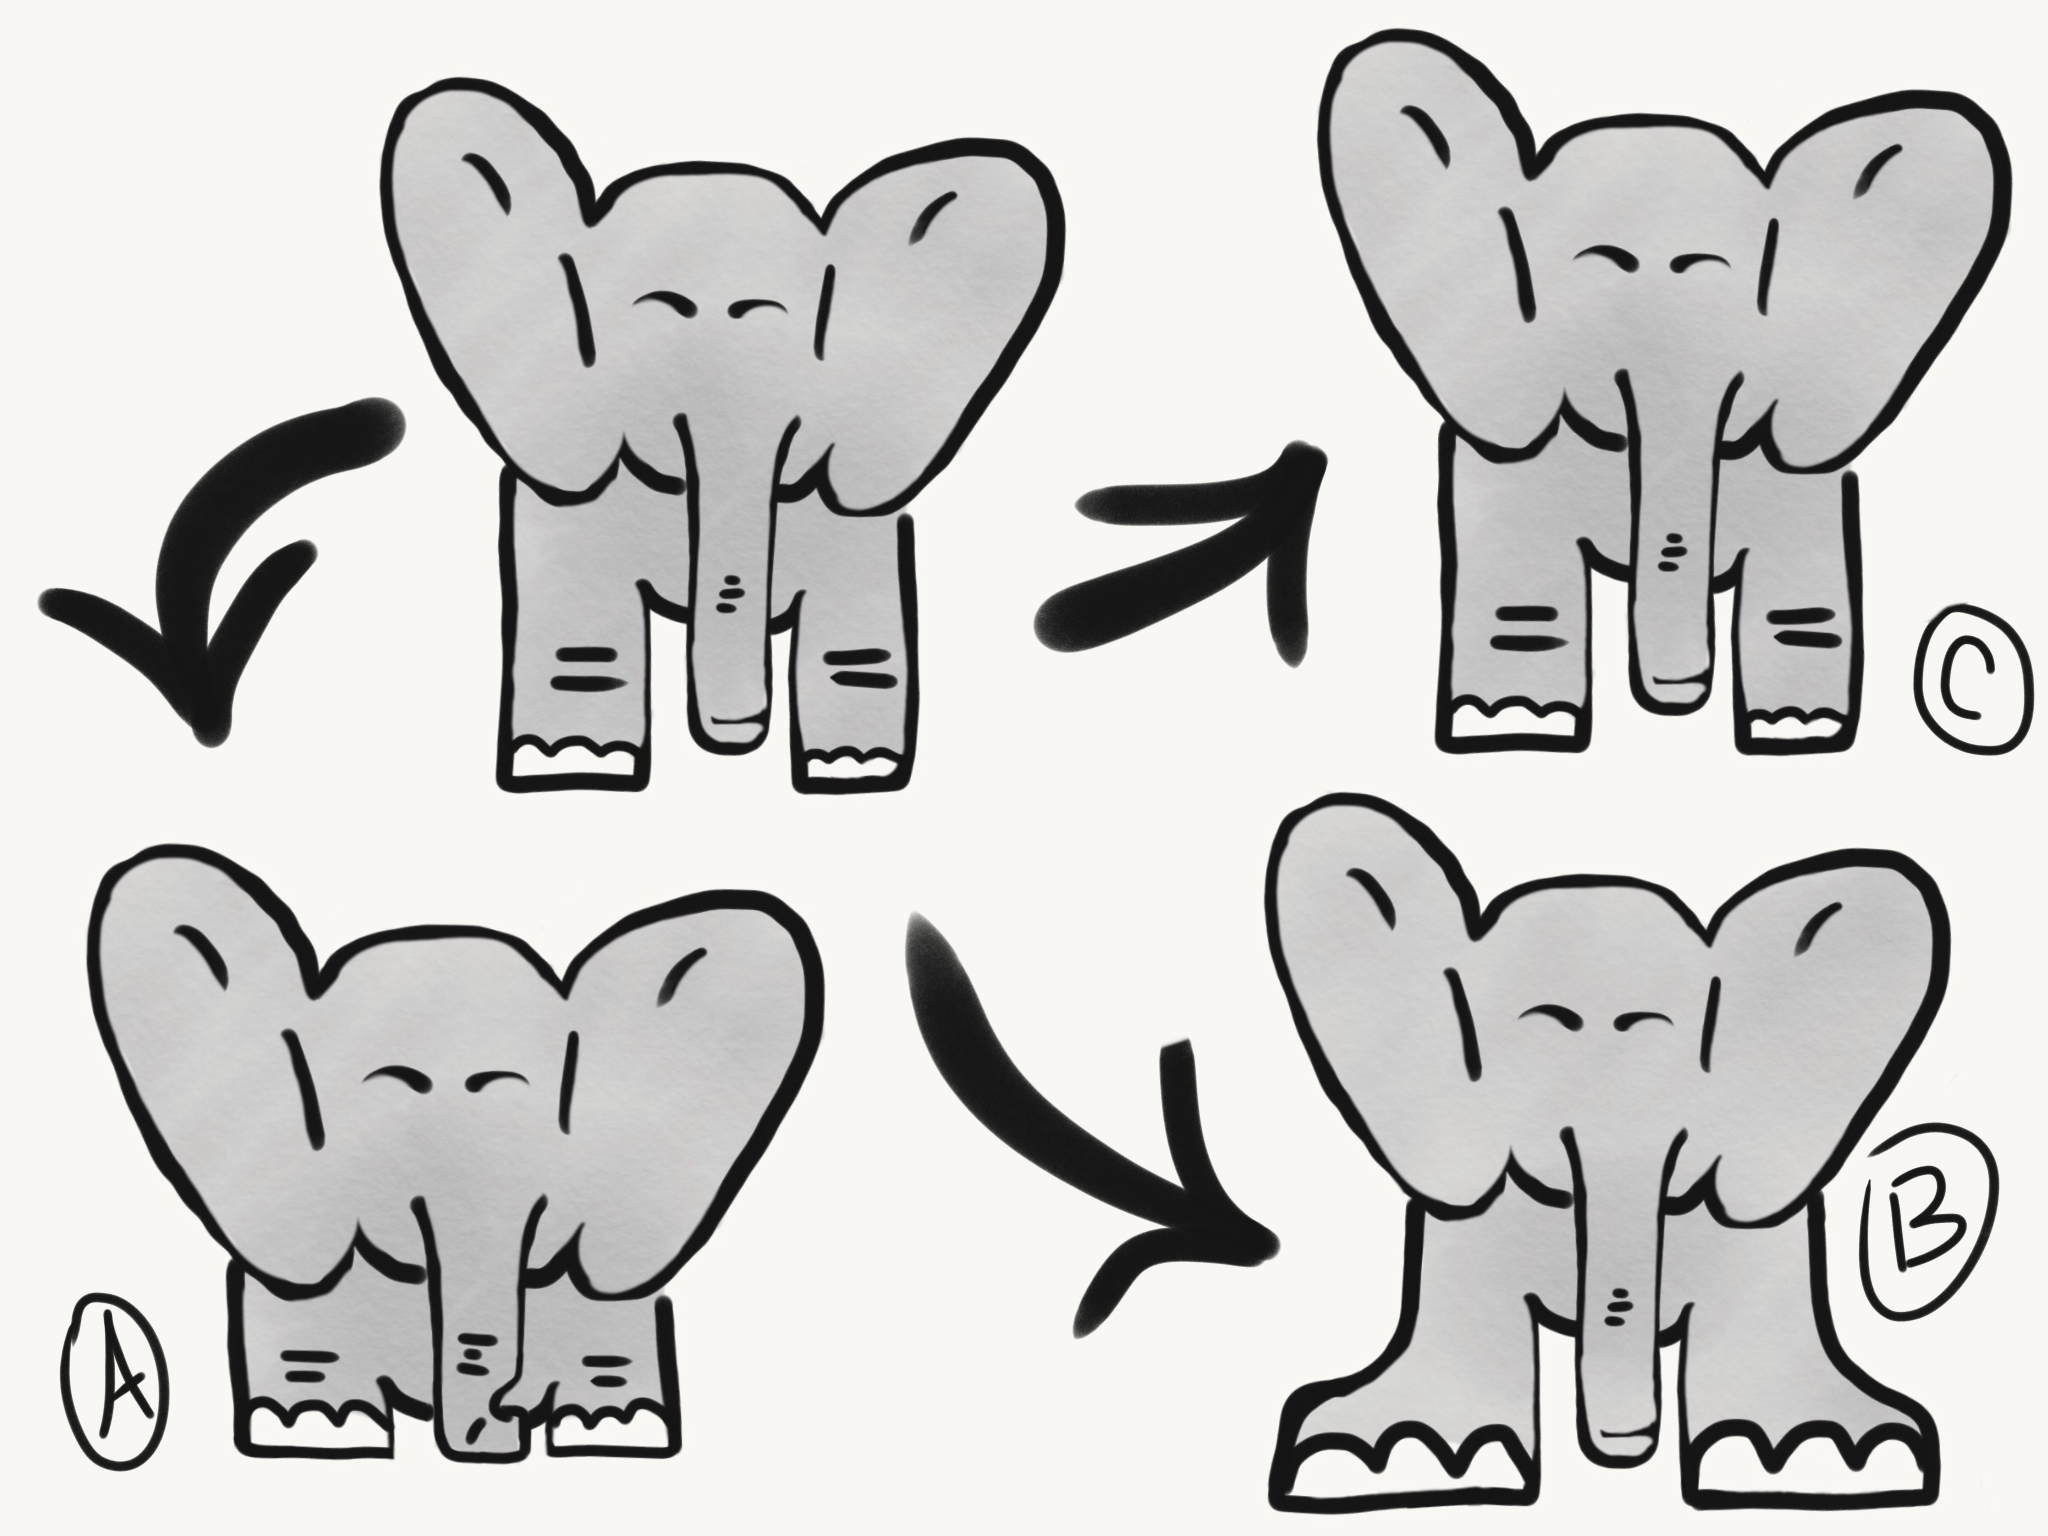
\includegraphics[width=\textwidth]{img/canalization_cartoon}
      \caption{canalization}
      \label{subfig:canalization}
    \end{subfigure}%
    \hfill
    \begin{subfigure}[b]{0.5\textwidth}
      \centering
      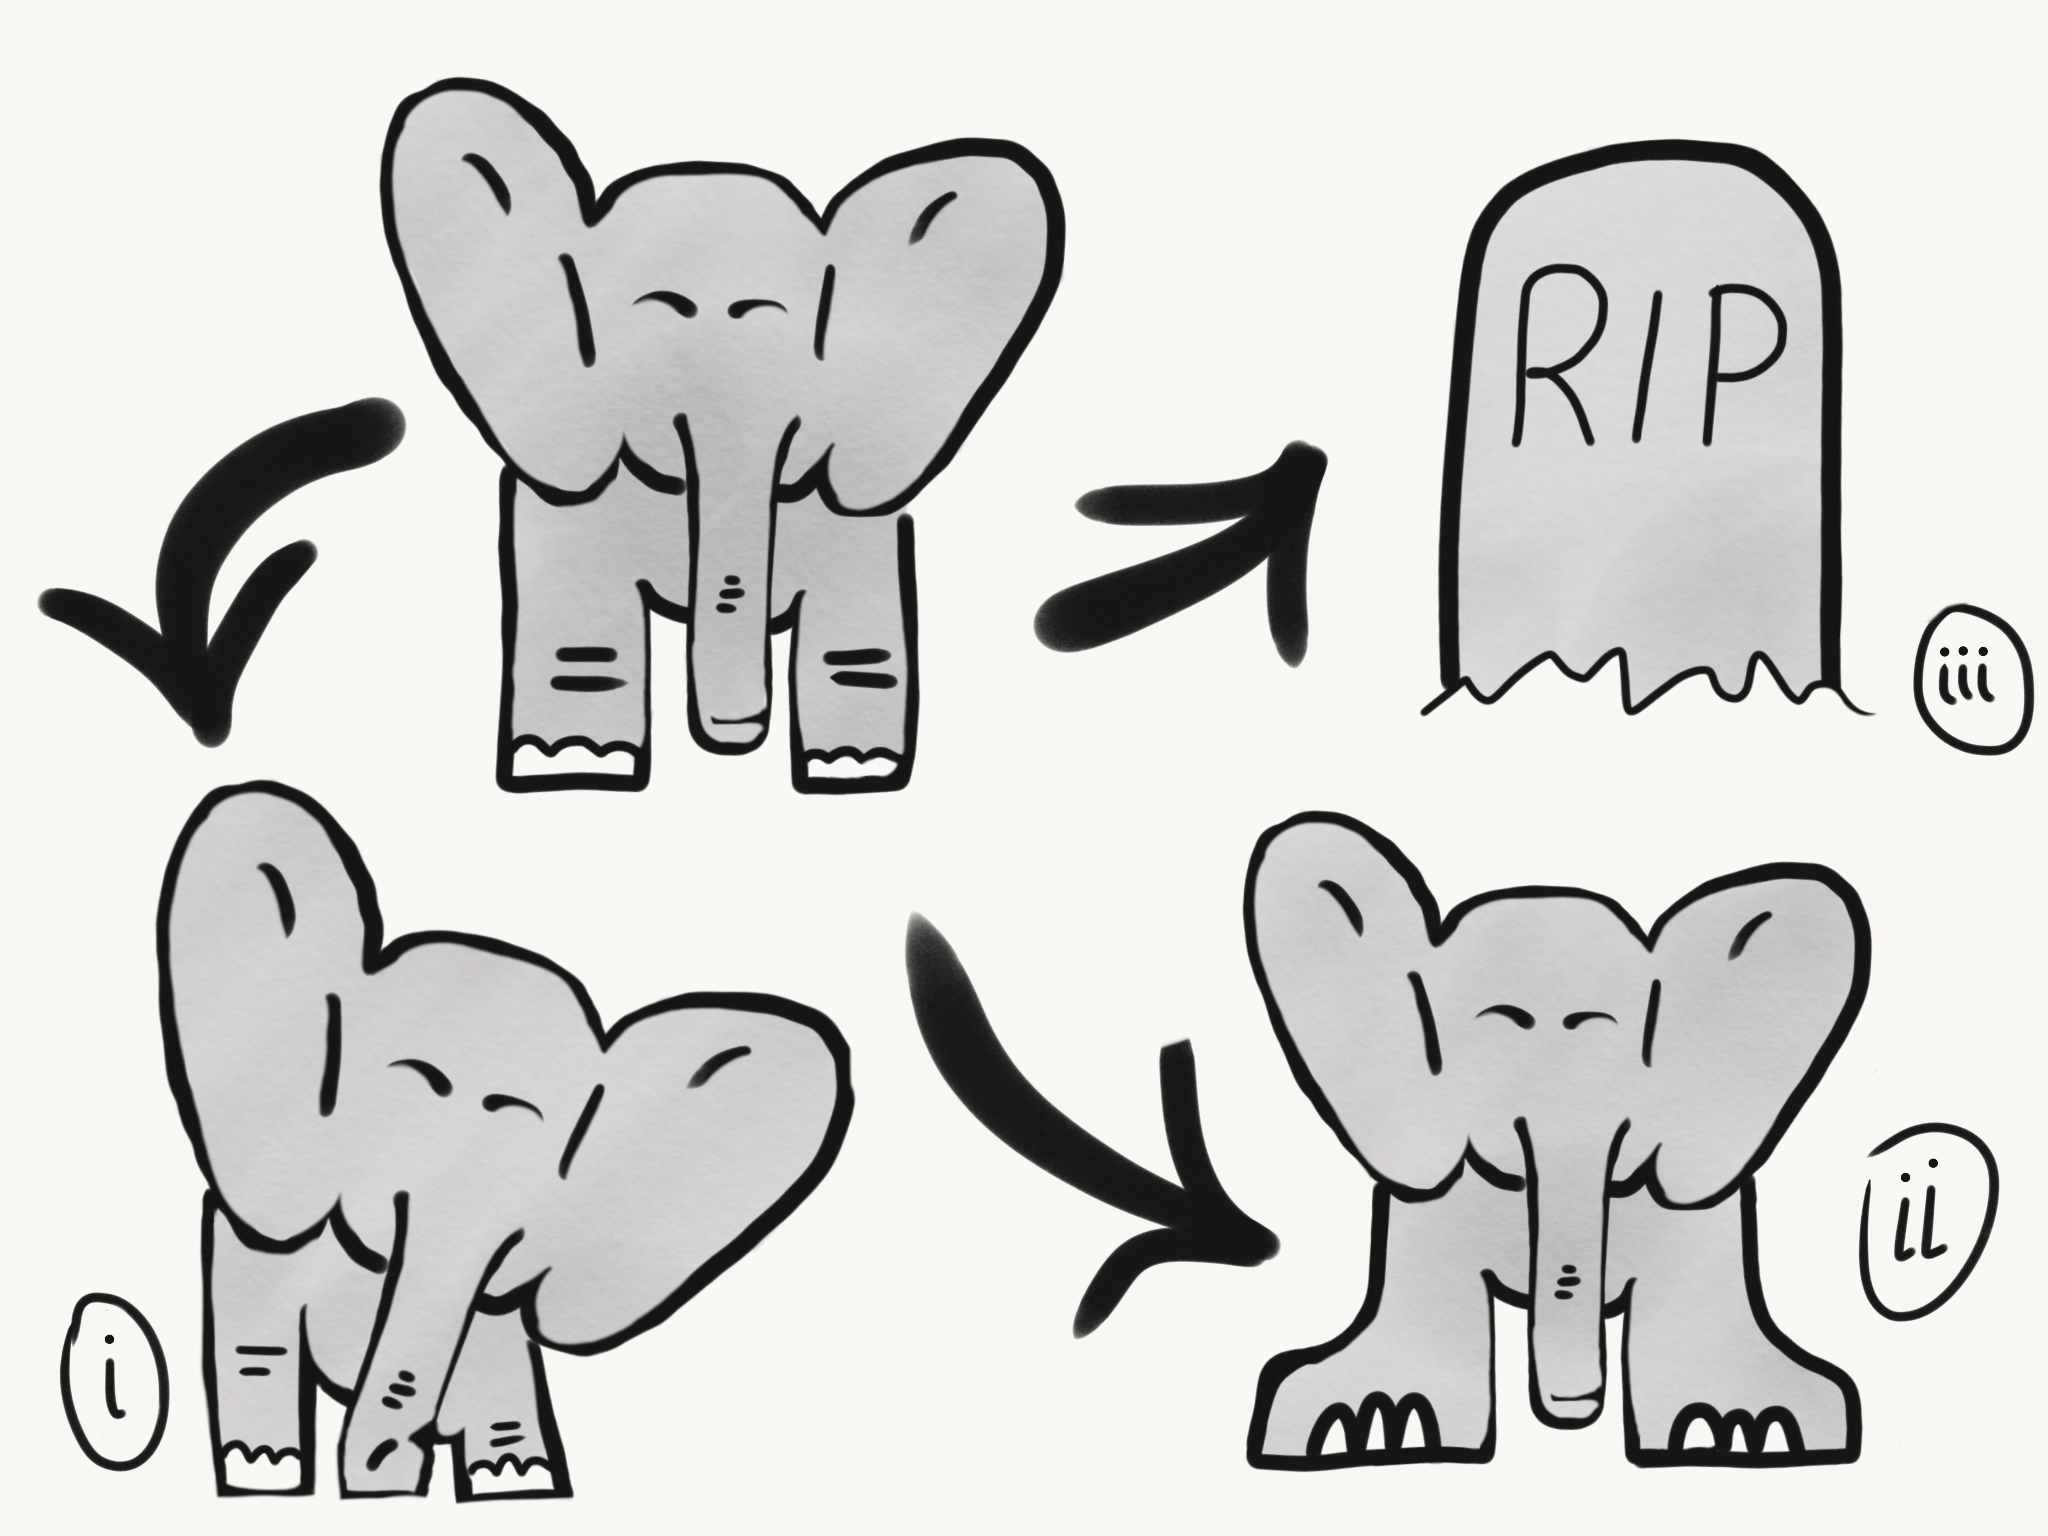
\includegraphics[width=\textwidth]{img/no_canalization_cartoon}
      \caption{non-canalization}
      \label{subfig:no_canalization}
    \end{subfigure}
 	\captionsetup{singlelinecheck=off,justification=raggedright}
    \vspace{-4ex}
  	\caption{a/i illustrates symmetry, b/ii illustrates grow-to-fit (exploratory growth \cite{Downing2015IntelligenceSystems}, c/iii illustrates robustness}
\end{figure}
\end{frame}

\begin{frame}{Inherent Bias: Regularity}
\begin{figure}
  \centering
  \begin{subfigure}[b]{0.5\textwidth}
    \centering
    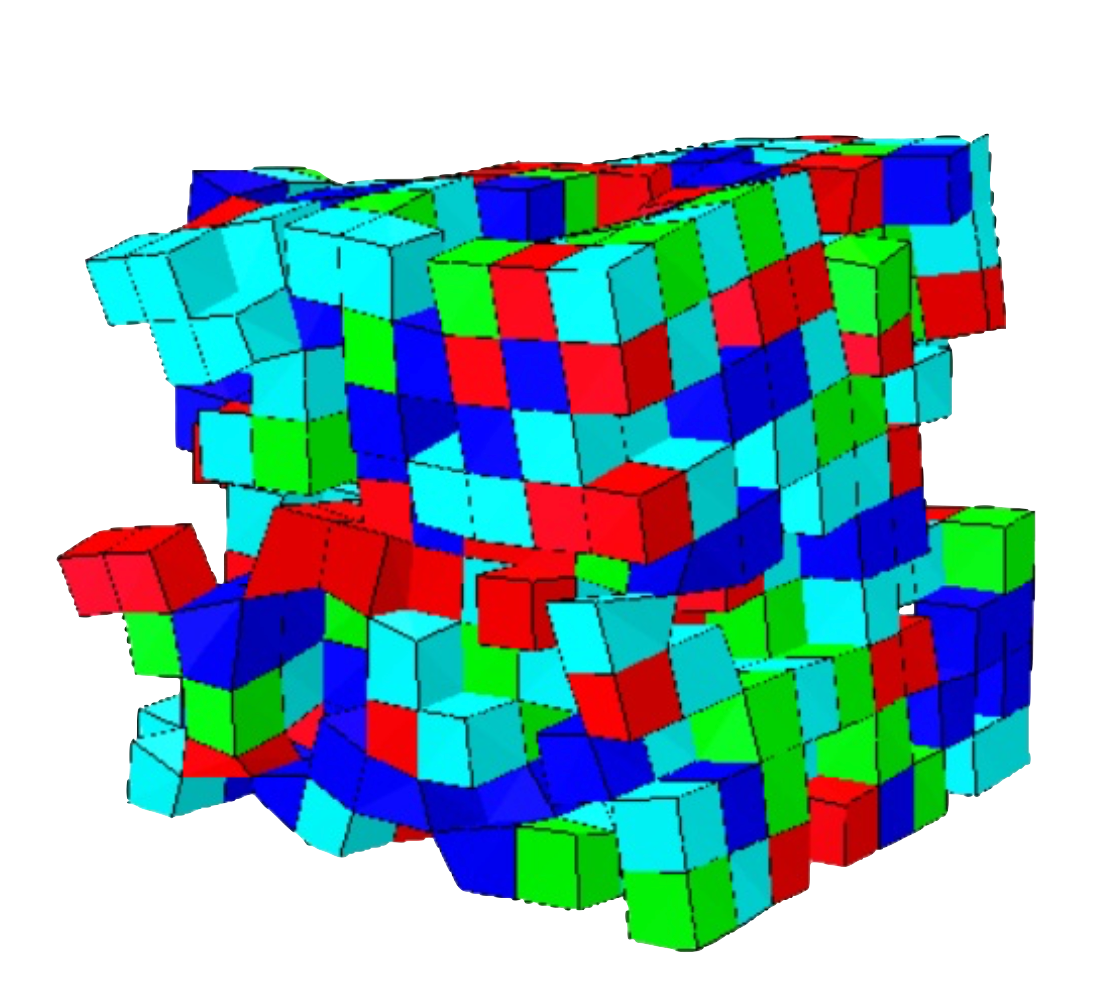
\includegraphics[width=\textwidth]{img/direct_encoding.png}
    \caption{direct encoding (low regularity)}
    \label{subfig:canalization}
  \end{subfigure}%
  \hfill
  \begin{subfigure}[b]{0.5\textwidth}
    \centering
    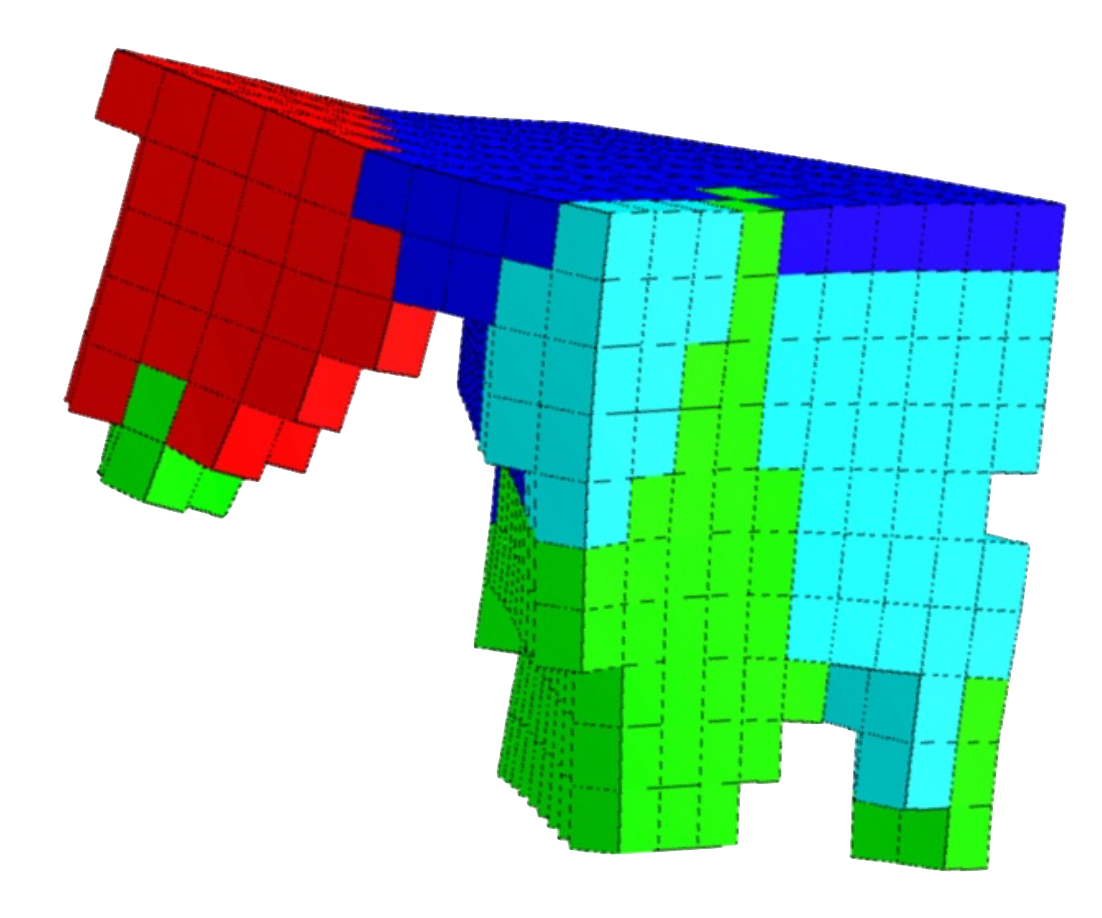
\includegraphics[width=\textwidth]{img/cppn-neat_encoded.png}
    \caption{indirect encoding (high regularity)}
  \end{subfigure}
  \captionsetup{singlelinecheck=off,justification=raggedright}
  \caption{words words words \cite{Cheney2013UnshacklingEncoding}}
\end{figure}
\end{frame}


\begin{frame}{Indirect Encodings}
\begin{figure}
  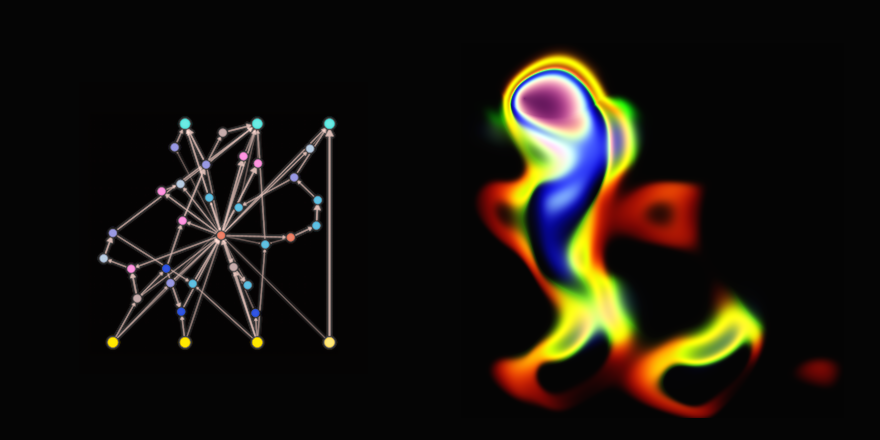
\includegraphics[width=\textwidth]{img/twitter_walking_fish.png}
  \captionsetup{singlelinecheck=off,justification=raggedright}  
  \caption{\cite{Ha2015Neurogram}}
\end{figure}
\end{frame}

\begin{frame}{Indirect Encodings}
\begin{figure}
  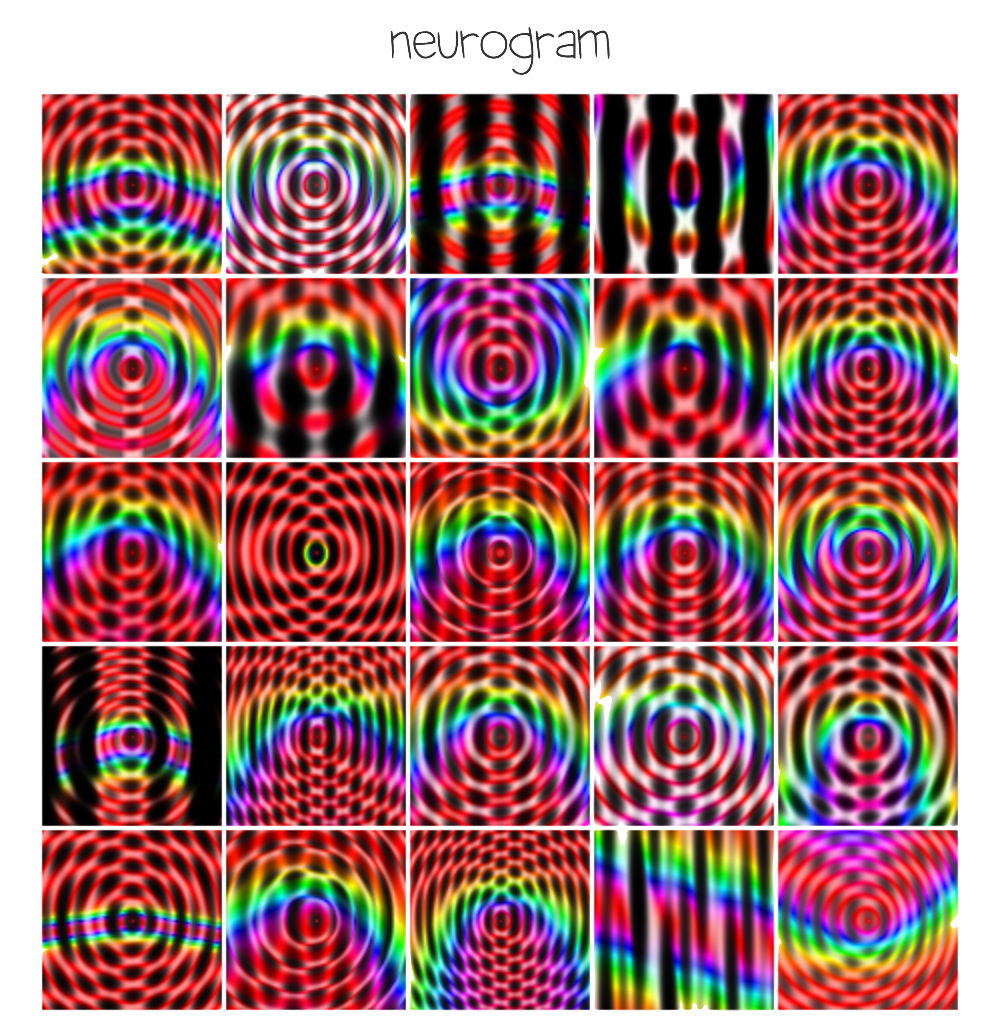
\includegraphics[width=0.6\textwidth]{img/neurogram.png}
  \captionsetup{singlelinecheck=off,justification=raggedright}
  \caption{\cite{Ha2015Neurogram}}
\end{figure}
\end{frame}

% \begin{frame}{Indirect Encodings}
% Genetic Regulatory Networks
% \begin{figure}
%   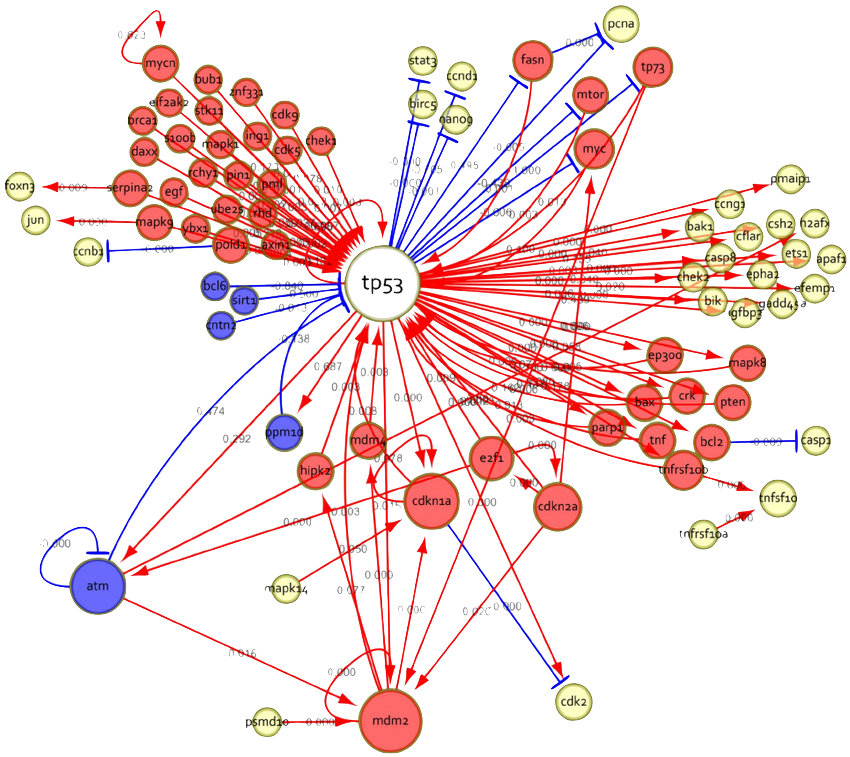
\includegraphics[width=0.5\textwidth]{img/gene_regulatory_network}
%   \captionsetup{singlelinecheck=off,justification=raggedright}
%   \caption{GRN example \cite{Chen2014AugmentingInference}}
% \end{figure}
% \end{frame}

